% !TeX spellcheck = en_US
\documentclass[conference]{IEEEtran}

% *** GRAPHICS RELATED PACKAGES ***
%
\usepackage[pdftex]{graphicx}
% declare the path(s) where your graphic files are
\graphicspath{{./figures/}}
% and their extensions so you won't have to specify these with
% every instance of \includegraphics
\DeclareGraphicsExtensions{.pdf,.jpeg,.png}

% *** MATH PACKAGES ***
%
\usepackage{amsfonts,amsmath,amssymb} % Mathematical symbols.

% correct bad hyphenation here
\usepackage{listings}
\usepackage{cite}
%\usepackage{caption}
\hyphenation{UPPAAL}

\usepackage{url}

\newcommand{\framework}[0]{\text{Gamma Framework}}
\newcommand{\Framework}[0]{\text{Gamma Framework}}
\renewcommand{\gamma}[0]{\text{Gamma}}
\renewcommand{\Gamma}[0]{\text{Gamma}}
\newcommand{\Yakindu}{\textsf{Yakindu}}

\newcommand{\eg}{e.g., }
\newcommand{\ie}{i.e., }

\newcommand{\RNum}[1]{\uppercase\expandafter{\romannumeral #1\relax}}
\newcommand{\ptolemy}{Ptolemy \RNum{2}}

\newcommand{\specialcell}[2][c]{%
	\begin{tabular}[#1]{@{}c@{}}#2\end{tabular}}

\newenvironment*{mytable}[3]{
	% #1: caption, #2: cimke, #3: oszlopdef		 
	\begin{table}[htbp]	
		\caption{#1}          
		\label{tab:#2}            
		\center%
		\begin{tabular}{#3}
		}
		{
		\end{tabular}
	\end{table}
}

% Define Language
\lstdefinelanguage{Gamma}
{
	% list of keywords
	morekeywords={
		const,
		integer, 
		natural,
		interface,
		extends,
		in,
		out,
		inout,
		event,
		import,
		package,
		statechart,
		rate,
		var,
		transition,
		from,
		to,
		region,
		initial,
		shallow,
		deep,
		history,
		state,
		entry,
		exit,
		assign,		
		sync,
		cascade,
		async, 
		of,
		port,
		provides,
		requires,
		component,
		bind,
		->,
		channel,
		-o)-,
		any,
		run,
		full,
		step,
		reset,
		priority,
		capacity,
		clock,
		s,
		ms,
		when,
		queue
	},
	sensitive=true, % keywords are not case-sensitive
	morecomment=[l]{//}, % l is for line comment
	morecomment=[s]{/*}{*/}, % s is for start and end delimiter
	morestring=[b]" % defines that strings are enclosed in double quotes
}

% Define Colors
\usepackage{color}
\definecolor{eclipseBlue}{RGB}{42,0.0,255}
\definecolor{eclipseGreen}{RGB}{63,127,95}
\definecolor{eclipsePurple}{RGB}{127,0,85}

\definecolor{lightgray}{rgb}{0.95,0.95,0.95}
\lstset{
	basicstyle=\footnotesize, % print whole listing small
	keywordstyle=\color{black}\bfseries, % bold black keywords
	identifierstyle=, % nothing happens
	% default behavior: comments in italic, to change use
	% commentstyle=\color{green}, % for e.g. green comments
	stringstyle=\scriptsize,
	showstringspaces=false, % no special string spaces
	backgroundcolor = \color{white},
	aboveskip=1.5\medskipamount,	
	columns=flexible,
	keepspaces=true,
	escapeinside={(*@}{@*)},
	captionpos=b,
	breaklines=true,
	frame=single,
	float=!ht,
	literate=*
	{á}{{\'a}}1	{é}{{\'e}}1	{í}{{\'i}}1	{ó}{{\'o}}1	{ö}{{\"o}}1	{ő}{{\H{o}}}1	{ú}{{\'u}}1	{ü}{{\"u}}1	{ű}{{\H{u}}}1
	{Á}{{\'A}}1	{É}{{\'E}}1	{Í}{{\'I}}1	{Ó}{{\'O}}1	{Ö}{{\"O}}1	{Ő}{{\H{O}}}1	{Ú}{{\'U}}1	{Ü}{{\"U}}1	{Ű}{{\H{U}}}1
}


% Set Language
\newcommand{\setGammaSyntax}{
	\lstset {
		language={Gamma},
		basicstyle=\footnotesize, % Global Code Style
		captionpos=b, % Position of the Caption (t for top, b for bottom)
		extendedchars=true, % Allows 256 instead of 128 ASCII characters
		tabsize=2, % number of spaces indented when discovering a tab 
		columns=fixed, % make all characters equal width
		keepspaces=true, % does not ignore spaces to fit width, convert tabs to spaces
		showstringspaces=false, % lets spaces in strings appear as real spaces
		breaklines=true, % wrap lines if they don't fit
		frame=trbl, % draw a frame at the top, right, left and bottom of the listing
		frameround=tttt, % make the frame round at all four corners
		framesep=4pt, % quarter circle size of the round corners
		%		numbers=left, % show line numbers at the left
		%		numberstyle=\tiny\ttfamily, % style of the line numbers
		commentstyle=\color{eclipseGreen}, % style of comments
		keywordstyle=\color{black}\bfseries, % style of keywords
		stringstyle=\color{eclipseBlue}, % style of strings
	}
}

\begin{document}
\setGammaSyntax
\title{The Composition Language of the \\ Gamma Framework}

% author names and affiliations
% use a multiple column layout for up to three different
% affiliations
\author{\IEEEauthorblockN{Bence Graics, Vince Moln\'ar}
\IEEEauthorblockA{Budapest University of Technology and Economics, \\
Department of Measurement and Information Systems \\
Budapest, Hungary \\
Email: \texttt{bence.graics@gmail.com},  \texttt{molnarv@mit.bme.hu}}

}

% make the title area
\maketitle

% As a general rule, do not put math, special symbols or citations
% in the abstract
\begin{abstract}
%	Many of today's safety-critical systems are reactive, embedded systems. Their internal behavior is usually represented by state-based models. Furthermore, as the tasks carried out by such systems are getting more and more complex, there is a strong need for compositional modeling languages. Such modeling formalisms start from the component-level and use composition to build the system-level model as a collection of simple modules.
%	There are a number of solutions supporting the model-based development of safety-critical embedded systems. One of the popular open-source tools is Yakindu, a statechart editor with a rich language and code generation capabilities. However, Yakindu so far lacks support for compositional modeling.
%	This paper proposes a formal compositional language tailored to the semantics of Yakindu statecharts. We propose precise semantics for the composition to facilitate formal analysis and precise code generation. Based on the formal basis laid out here, we plan to build a complete tool-chain for the design and verification of component-based reactive systems.
\end{abstract}

% For peer review papers, you can put extra information on the cover
% page as needed:
% \ifCLASSOPTIONpeerreview
% \begin{center} \bfseries EDICS Category: 3-BBND \end{center}
% \fi
%
% For peerreview papers, this IEEEtran command inserts a page break and
% creates the second title. It will be ignored for other modes.
\IEEEpeerreviewmaketitle

\section{Introduction}

Statecharts \cite{Harel:1987:SVF:34884.34886} are a popular formalism to describe the behavior of reactive systems, which process stimuli from the environment and react with respect to their internal states. Statecharts introduce complex elements to aid the modeling of such systems, e.g., variables, hierarchical state refinement, history states and complex transitions (e.g., inner transitions).

The requirements such systems have to meet are getting more complex, which can result in very large system models, encumbering verifiability, maintenance and extensibility. A well-known solution for managing complexity is decomposition. In case of statecharts, one way of decomposition is to define individual reactive components that, by means of some communication, realize a more complex behavior. There are a number of modeling tools that aim to support this practice with various model-driven software development techniques such as code generation and verification.

The Gamma Statechart Composition Framework is one such tool, providing a layer for composing individual statechart components (possibly coming from other tools) while extending the capabilities of automatic code generation and verification and validation (V\&V). In this paper, we introduce the new composition language of Gamma that enables the hierarchical mixing of different composition semantics, with a focus on features and modeling aspects.

\textbf{Asynchronous-reactive:} Such models represent a set of components that are executed independently. Asynchronous components communicate with each other by means of messages and message queues. This semantics is convenient when decomposition is both logical and physical, \eg for the design of communicating microservices running in different processes.
	
\textbf{Synchronous-reactive:} A synchronous model represents a coherent unit with a single functionality consisting of concurrently (but not independently) running components. Contained components communicate in a synchronous manner using signals. This semantics is suitable for the logical decomposition of systems or the modeling of hardware-related designs.
	
\textbf{Cascade:} Cascade models represent a set of filters that are applied sequentially to derive an output from an input. Like synchronous-reactive components, cascade components also facilitate the logical decomposition of a problem, but it focuses more heavily on process-like models. Therefore, this model supports the design of adapters, runtime monitors and units with a batch-like execution.

The rest of the paper is structured as follows. Section~\ref{sec:related-tools} presents a short summary of tools that inspired the design of the composition language. The elements of a the language itself and an example are introduced in Section \ref{sec:composition-language}. Finally, Section \ref{sec:conclusion} provides concluding remarks and ideas for future work.

\section{Related Tools}
\label{sec:related-tools}

\ptolemy\footnote{\url{http://ptolemy.eecs.berkeley.edu/}} \cite{ptolemy,ptolemy2} is an open-source software framework, aiming to support
the modeling of hierarchical composite systems. It supports system design with numerous component variants and communication semantics. Communication semantics of interactive components are determined by \emph{directors}, which are responsible for defining a \emph{model of computation} on a particular hierarchy level. Various directors (e.g., process network, synchronous data flow
or synchronous reactive) through different hierarchy levels can be combined, facilitating the design of complex model behavior. One of the main strengths of Ptolemy II is the simulation capability of designed models. However, source code generation from models is not supported and it does not provide formal verification capabilities either.

BIP\footnote{\url{http://www-verimag.imag.fr/Rigorous-Design-of-Component-Based.html?lang=en}} \cite{bip,bip3} is a modeling framework that focuses on the formal definition of heterogeneous systems.
BIP offers a language to define hierarchical composite models, where the interactions of constituent components are based on \emph{synchronization}. BIP defines a clear operational semantics that describes the behavior for both atomic components (transition system model) and compound components (rigorous interaction rules of contained components). BIP offers a comprehensive tool set, which provides model transformers for third-party models, e.g., MATLAB/Simulink, code generators to produce C/C++ code, and formal
verification capabilities of defined BIP models.

Stateflow\footnote{\url{https://www.mathworks.com/products/stateflow.html}} \cite{stateflow} is a commercial framework that supports the modeling of
reactive systems. Stateflow supports the design of composite
statecharts by combining
statechart diagrams with flowchart diagrams and providing various scheduling
algorithms. Furthermore, Stateflow supports the simulation, validation and verification of created models as well as source code generation. Stateflow is a mature software with professional
support. Unfortunately, as Stateflow is a commercial product, its study and extension is cumbersome, which is not favorable in research context. Also, commercial licenses are expensive.


%\section{The Gamma Statechart Language}
%\label{sec:statechart-language}
%The goal of the \gamma\ statechart language is to support the rigorous design of reactive
%systems while providing conventional facilities of modern statechart languages. To support
%strictness, a well-defined semantics is needed. The language is given a denotational semantics
%described in \cite{graics-bence-bsc} by mapping gamma model constructions to the elements of a formal timed
%automaton implementation. The most important elements of the language are presented in this section using a simple \emph{timer} statechart capable of measuring time.
%
%The execution of the statechart starts in the \textsl{Idle} state, with the \textsl{elapsedTime} variable set to $-1$. When a \textsl{start} event is received on its \textsl{control} port, it changes its state to \textsl{Measuring}, where the incoming \textsl{tick} events are counted using a loop transition. When a \textsl{stop} event is received, the statechart goes back to state \textsl{Idle} while storing the elapsed number of ticks in variable \textsl{elapsedTime}. The measuring process can be restarted with an additional \textsl{start} event.
%\begin{lstlisting}
%statechart Timer [
%  // Port for communication
%  port control : provides Control
%] {
%  var elapsedTime : integer := -1
%  // Transition without trigger
%  transition from Initial to Idle 
%  // Transitions with triggers
%  transition from Idle to Measuring
%    when control.start / assign elapsedTime := -1
%  transition from Measuring to Measuring
%    when control.tick && !(control.stop)
%  transition from Measuring to Idle
%    when control.stop
%  // Main region
%  region main {
%    // Initial state
%    initial Initial
%    // Simple state
%    state Idle
%    // Simple state with entry action
%    state Measuring {
%      entry / assign elapsedTime := elapsedTime + 1
%    }		
%  }
%}
%\end{lstlisting}
%
%Statecharts communicate with their environment via \textsl{ports} using \textsl{events}. A port realizes an \textsl{interface} in either required or provided mode, which determines the event types that can be dispatched or received through the particular port. The language supports the definition of \textsl{variables} with the following types: integer, natural, real, boolean and enumeration types. Variables can be used in guard expressions and assignment expressions of \textsl{transitions}. Events of ports can also be raised by transitions.
%
%One of the unique features of the \gamma\ statechart language is the \textsl{complex trigger}. A complex trigger, consisting of simple triggers, can describe the relation
%of multiple triggers as logical relations. A complex trigger may initiate a particular execution only if the corresponding logical relation is evaluated to true. Furthermore, an execution can be
%initiated on the absence of a certain event.
%
%\textsl{Region} is the container element of node elements. A region can either be a top region, contained by a statechart or a subregion,
%contained by a composite state. A region must contain a single entry state, which can be an \textsl{initial state} (no history), a \textsl{shallow history} or \textsl{deep history state}. \textsl{States} can have \textsl{entry} and
%\textsl{exit events}, which specify different actions that have to be taken when the state is activated
%or deactivated, respectively. \textsl{Composite states} extend simple states with the ability of containing
%one ore more regions. If a particular state contains multiple regions, they are parallel.

\section{The Gamma Composition Language}
\label{sec:composition-language}
The gamma composition language supports the definition of communicating composite models
built from individual reactive components. The design of composite systems starts with the definition of interfaces, which define the possible event types that can be transmitted between components. The interfaces then can be realized by ports of components, which can be connected, thus enabling communication. Communicating components can be wrapped by composite models, creating an independent composite reactive unit with rigorously defined interaction patterns.

\subsection{Communication Elements}
Interfaces serve as contracts between
interacting components of \gamma\ models. These contracts apply to the ability of dispatching
and receiving certain events. Events represent occurrences of some importance. Directions of events can be in, out or in-out;
the latter represents events that can be used as both in and out events. Events can contain
parameter declarations, which provide additional information about the corresponding event. An example interface definition can be seen below.
\begin{lstlisting}
interface LightCommands {
  out event displayRed
  out event displayGreen
  out event di splayYe l low
  out event displayNone
}
interface PoliceInterrupt {
  out event police
}
\end{lstlisting}

Ports serve as endpoints of component instances in a composite component model,
through which events can be dispatched or received. In \gamma\ models, communication between component
instances always happens through ports. Events are either called signals in case of
synchronous components or messages in case of asynchronous components. Each port realizes
a single interface in either provided or required mode. In provided mode ports dispatch and receive events according to the direction specified in the event declarations. In case of required mode, interfaces are ``turned inside out'', i.e., events declared with the direction in will be
dispatched, and events declared with the direction out will be received through such ports. Note that if two ports realize the same interface, one of them in provided mode, the other
one in required mode, they can be connected since the direction of the events would match. Note that
the realization mode does not specify a single direction in which events are transmitted
through the particular port – dispatch and reception can be mixed in both cases. A port is considered as a broadcast port if the interface realization mode is provided and
the realized interface contains only out events. Unlike other ports, a broadcast port can
be connected to multiple ports realizing the same interface in required mode.

The concept of ports realizing interfaces in providing or requiring modes may be unusual to
some designers, since ports usually support one-way event transmission in modern modeling
languages. Our goal with this solution is to investigate the possibilities residing in interface-based
communication in the domain of reactive systems. On the other hand, it is possible to
use only out events on every interface -- then provided mode is ``output'' mode and required
mode is ``input'' mode.


\subsection{Components}

\subsection{Composite Models}

\subsection{Summary}
As a summary, Table \ref{tab:supported-component-types} describes the component types that are supported by the \gamma\ composition language in terms of \emph{synchronousness} and \emph{compositeness}.

\begin{mytable}{Component types supported by the \gamma\ composition language.}{supported-component-types}{|c||c|c|}
	\hline
	& \textbf{Atomic} & \textbf{Composite} \\ \hline \hline
	%	1 & Equality & equal & equality & Right-to-left  \\ \hline
	\textbf{Synchronous} & Statechart & \specialcell{Synchronous composite component \\ Cascade composite component}\\ \hline
	\textbf{Asynchronous} & Synchronous component wrapper & \specialcell{Asynchronous composite component}\\ \hline
\end{mytable}

Figure \ref{fig:gamma-object-tree} presents the containment hierarchy of an example composite model. Note that the synchronous and asynchronous domain can be bridged only by synchronous composite wrappers. Furthermore, the leaves, which generally define the behavior of composite components, are always statechart definitions.

\begin{figure}[htbp]
	\center
	%	\resizebox{140mm}{!}{
	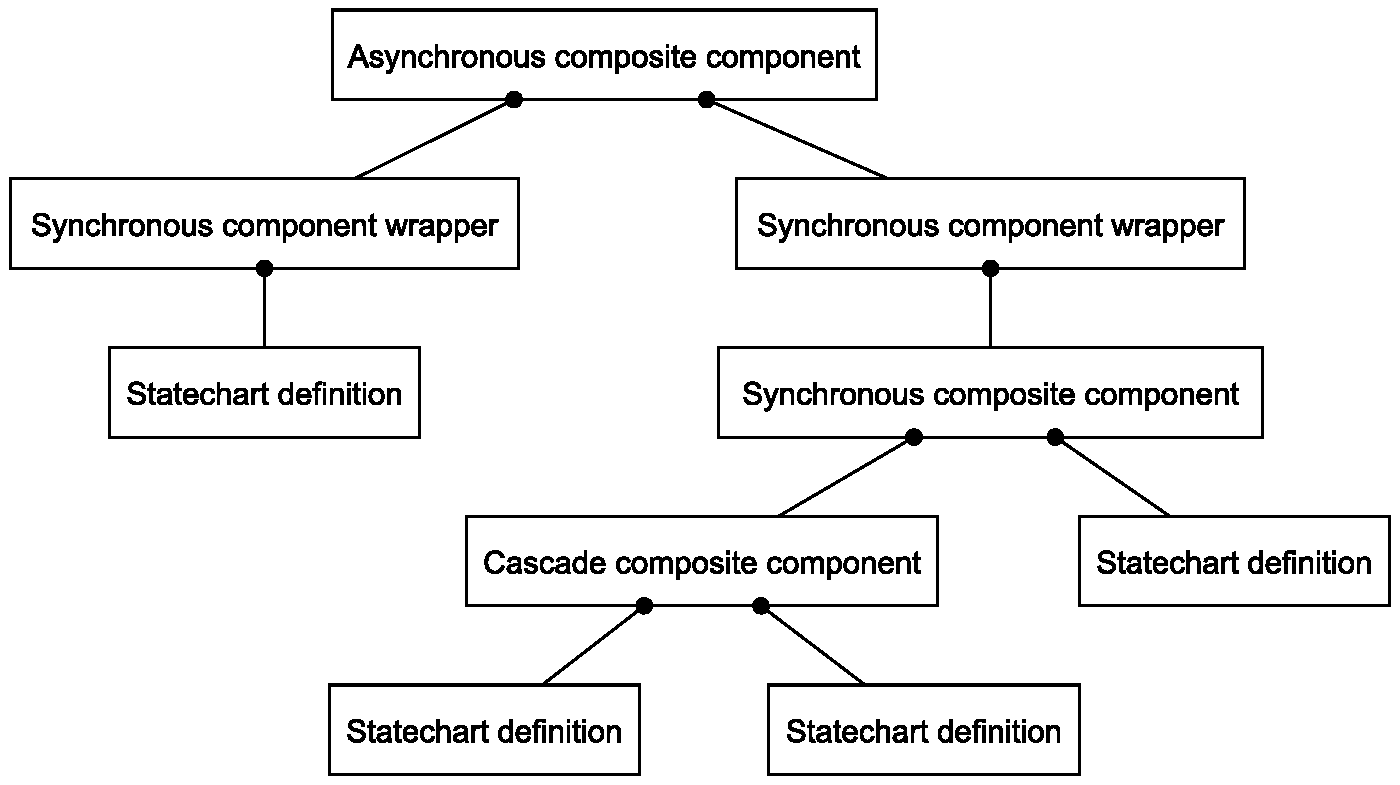
\includegraphics[width=1.0\linewidth]{figures/gamma_object_tree.pdf}
	%	}
	\caption{A composite model hierarchy in \gamma.}
	\label{fig:gamma-object-tree}
\end{figure}

\subsection{Example}

\begin{lstlisting}
import trafficLight
import controller

sync Crossroad [
  // External ports of the composite model
  port police : requires PoliceInterrupt,
  port priorityLightOutput : provides LightCommands,
  port secondaryLightOutput : provides LightCommands
] {
  // Component instances
  component controller : Controller
  component priorityLight : TrafficLight
  component secondaryLight : TrafficLight
  // Bindings of system ports to internal ports
  bind police -> controller.policeInterrupt
  bind priorityLightOutput -> priorityLight.lightCommands
  bind secondaryLightOutput -> secondaryLight.lightCommands
  // Channel definitions connecting internal ports
  channel [controller.priorityControl] -o)- [priorityLight.control]
  channel [controller.secondaryControl] -o)- [secondaryLight.control]

  channel [controller.priorityPolice] -o)- [priorityLight.policeInterrupt]
  channel [controller.secondaryPolice] -o)- [secondaryLight.policeInterrupt]
}
\end{lstlisting}

\begin{figure}[!h]
	\centering
	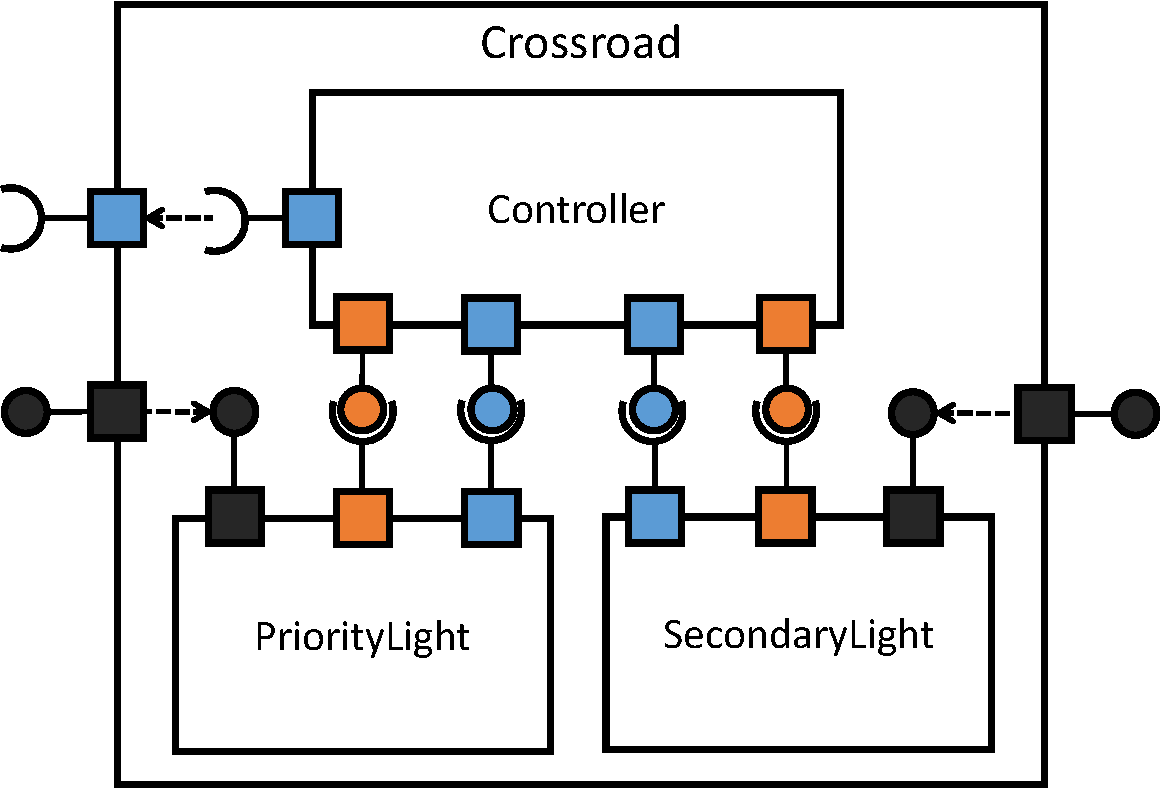
\includegraphics[width=0.52\textwidth]{figures/Controller-gcd.pdf}
	\caption{The synchronous Crossroad composite model composing a Controller and two Traffic light statecharts.}
	\label{fig:block_diagram_cropped2}
\end{figure}

\section{Conclusion and Future Work}
\label{sec:conclusion}

%\section{Language for Composition}
%\label{sec:compositional_language}
%%The compositional language is based on Xtext\footnote{http://eclipse.org/Xtext/} due to its easy-to-use language and the additional features it provides, e.g.~a parser, a linker, a compiler and content assist.
%
%This section defines the syntax of the compositional language and introduces the semantics the composite system conforms to. This semantics is heavily influenced by the statechart semantics defined by \Yakindu\ and strives to address some of its problems, e.g.~gives the ability to parallel regions to communicate with each other. 
%
%\subsection{Syntax}
%
%Figure \ref{fig:metamodel} depicts the metamodel of the compositional language. The root element in the metamodel is the \textsl{System}. A \textsl{System} contains \textsl{Components} which refer to \Yakindu\ statecharts as well as \textsl{Instances} of such \textsl{Components}. Each \textsl{Component} has an \textsl{Interface} that contains \textsl{Ports}. Through \textsl{Ports}, signals of statecharts can be transmitted or received according to their directions.
%
%\textsl{Channels} can be used for defining the emergent behavior of the composite system. A \textsl{Channel} has one or more \textsl{Inputs} and one or more \textsl{Outputs}. An Input of a \textsl{Channel} connects to an output \textsl{Port} of an \textsl{Instance} and vice versa. Whenever a \textsl{Channel} receives a signal through any of its \textsl{Inputs}, the signal is sent to each \textsl{Output}, i.e.~to the corresponding input \textsl{Ports} of \textsl{Instances}. The language does not support connecting \textsl{Ports} of the same direction and a validation rule is defined that marks incorrect connections.
%
%The language supports the definition of an interface through which the composite system interacts with its environment. This is the \textsl{SystemInterface} that contains \textsl{SystemPorts}. \textsl{SystemPorts} are aliases of \textsl{Ports} of  \textsl{Instances}. If a signal arrives to a \textsl{SystemInPort}, it will be forwarded to the \textsl{Port} of the referred \textsl{Instance} instantly. \textsl{SystemOutPorts} work similarly, but with output \textsl{Ports} of \textsl{Instances}. 
%%
%%\begin{itemize}
%%	
%%	\item Components: A Component refers to a \thetatool\  Statechart specification. For each Component an Interface has to be defined.
%%	
%%	\item Interface: An Interface of a Component is composed of Ports. An Interface does not need to have a Port declaration for each \thetatool\ Signal declaration defined in the Statechart specification. 
%%	\item Port: Ports are endpoints the Instances of the particular Component will send or receive signals on. A Port refers to a \thetatool\ Signal declaration and it also has a direction (IN or OUT). A Port with the direction of IN may only \emph{receive} signals, OUT ports are for \emph{transmitting} signals. A Signal declaration referred to by a Port may have a type. This means values can be transmitted through signals. 
%%	
%%	\item Instances: Instances can be instantiated of Components. A Component may have multiple instantiations or none at all.
%%	\item Channels: Connecting Ports of multiple instances can be defined using Channels. A Channel has one or more Inputs and one or more Outputs. An Input consists of an Instance and a Port with the direction of OUT. An Output is similar to an Input, but their Ports are with the direction of IN. Whenever a Channel receives a signal through any of its Inputs, the signal is sent to each Output, which means all Instances connected to the particular Channel will get the signal. Connecting Ports of the same direction is not possible. Ports referring to Signal declarations with different types may not be connected. 
%%	\item System Interface: The System under design has an Interface. This System Interface consists of zero or more System IN Ports and zero or more System OUT Ports. 
%%	\item System Ports: An IN/OUT Port of the system is an alias of an IN/OUT Port of one of its Instances that is visible on the Interface of the System. For instance, if a signal arrives to an IN Port of the system, it will be forwarded to the corresponding Port of the specified Instance instantly (in the same step).
%%\end{itemize}
%
%For ease of understanding, an example is presented that defines a composition of statecharts using the specified compositional language. The system consists of two \textsl{Components}, \emph{CoffeMachineComponent} and \emph{LightComponent} referring to a coffee machine (CoffeMachine) statechart and a light switch (LightSwitch) statechart, respectively. CoffeMachine has signal declarations for turning it on and off, for ordering a cappuchino and for putting its light on and off. A LightSwitch models a lamp that can be turned on and off.   
%%\captionsetup[lstlisting]{format=listing,singlelinecheck=false, margin=0pt, font={sf}}
%\begin{lstlisting}[basicstyle=\small]
%// System interface definition
%interface {
%    in {
%        on : machine.on
%        off : machine.off
%        cappuchino : machine.cappuchino
%    }
%}
%
%// Component interface definitions
%CoffeeMachine CoffeMachineComponent {
%    interface {
%        on : IN on
%        off : IN off
%        cappuchino : IN cappuchino
%        lightOn : OUT flashLight
%        lightOff : OUT turnOffLight 
%    }
%}
%
%LightSwitch LightComponent {
%    interface {
%        on : IN onButton
%        off : IN offButton
%    }
%}
%
%// Component instantiations
%CoffeMachineComponent machine
%LightComponent light
%
%// Channel definitions
%channels {
%    [machine.lightOn] -> [light.on]
%    [machine.lightOff] -> [light.off]
%} 	 
%\end{lstlisting}
%
%\begin{figure}[!t]
%	\centering
%	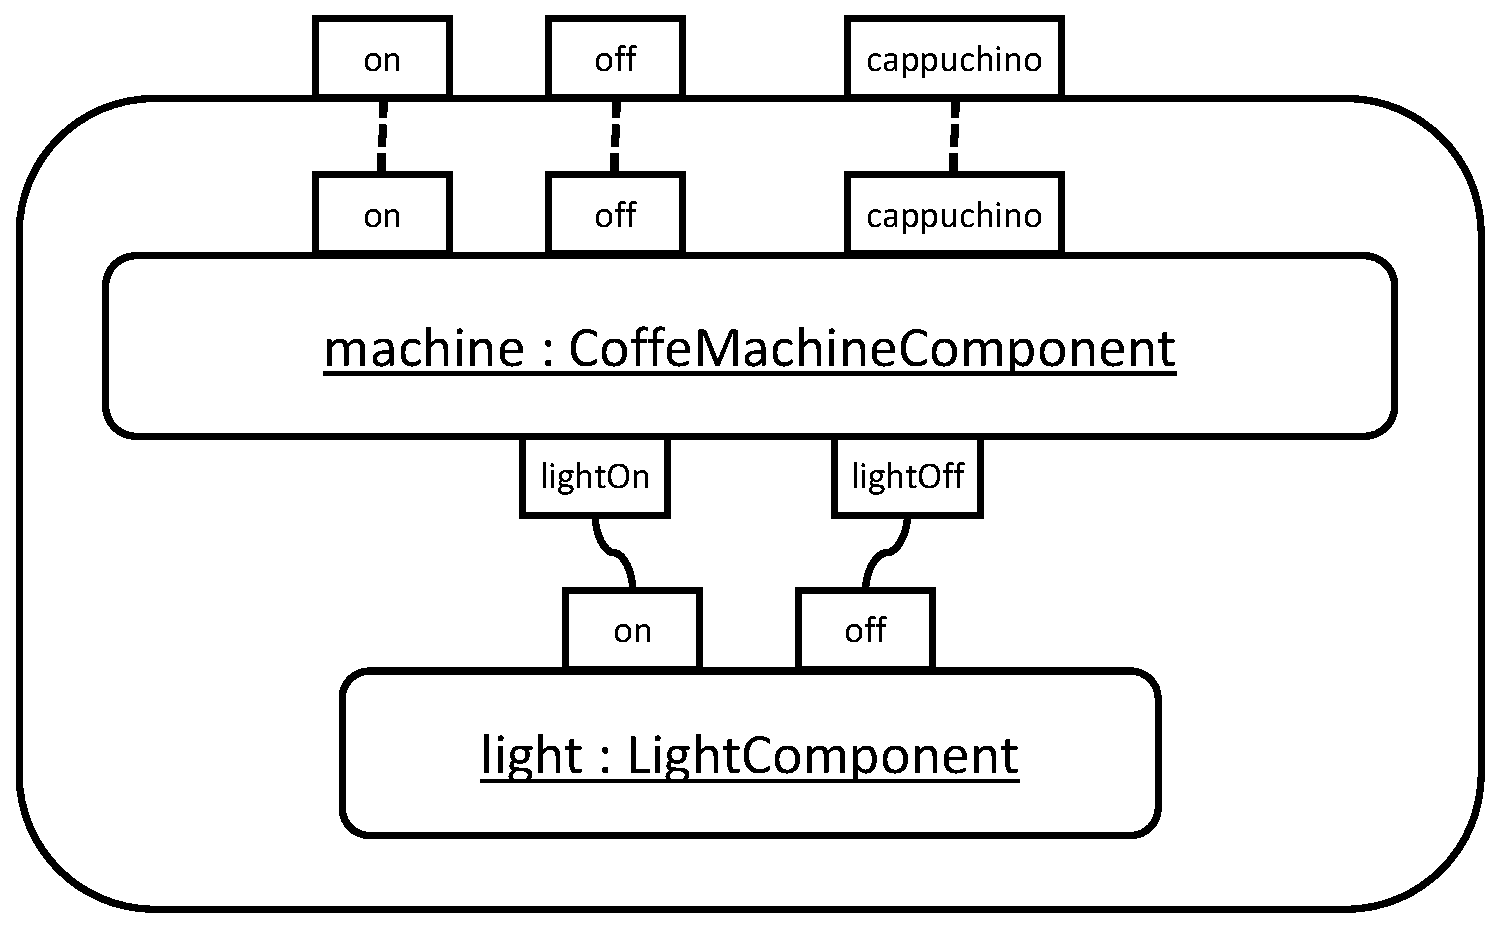
\includegraphics[width=0.455\textwidth]{figures/block_diagram_cropped2.pdf}%
%	\caption{A composite system of a CoffeMachine and a LightSwitch statechart.}
%	\label{fig:block_diagram_cropped2}
%\end{figure}
%
%Note that a composite system description constists of the following parts:
%
%\begin{itemize}
%	\item System interface definition: All input \textsl{Ports} of \emph{machine} are published to the interface of the system enabling the users to turn \emph{machine} on and off or order a cappuchino.
%	
%	\item Component interface definitions: \emph{CoffeMachineComponent} refers to \emph{on}, \emph{off} and \emph{cappuchino} through input \textsl{Ports} (denoted by the IN keyword) and \emph{flashLight}, \emph{turnOffLight} through output \textsl{Ports} (denoted by the OUT keyword). Both signal declarations of LightSwitch are referred to by input \textsl{Ports}.
%	
%	\item Component instantiations: Both \textsl{Components} are instantiated: \emph{machine} and \emph{light}.
%	
%	\item Channel definitions: The output \textsl{Ports} of \emph{machine} are connected to the input \textsl{Ports} of \emph{light}, making it possible for \emph{machine} to turn on \emph{light} at choice.
%\end{itemize}
%
%Figure \ref{fig:block_diagram_cropped2} depicts the composite system described by the previous code section.  Note that the individual components of the system are encapsulated. Interactions can be specified only through the defined interface.
%
%\subsection{Semantics}
%\label{sec:semantics}
% During the design of the semantics one of our goal was to define a language that enables the reuse of the source code generator of \Yakindu. Therefore the semantics of supported \Yakindu\ statecharts elements had to be considered, most importantly event raising.
%
%This section introduces the semantics of the compositional language.
%The compositional language enables to create a \emph{composite system}, that is formally a 4-tuple: $C = \langle\mathit{SC}, \mathit{CA}, \mathit{IN}, \mathit{OUT}\rangle$ where:
%
%\begin{itemize}
%	\item $\mathit{SC} = \{\langle S_1, s_1^0, T_1, I_1, O_1\rangle, \cdots, \langle S_n, s_n^0, T_n, I_n, O_n\rangle\}$ is a finite set of state machines.
%	
%	\item $I = \bigsqcup_{j = 1}^{n}I_j$, i.e.~the union of all in events of state machine components
%	
%	\item $O = \bigsqcup_{j = 1}^{n}O_j$, i.e.~the union of all out events of state machine components
%	
%	\item $\mathit{CA} \subseteq 2^O \times 2^I$, i.e.~channel associations relate a finite set of outputs to a finite set of inputs
%	
%	\item $\mathit{IN} \subseteq I $, i.e.~the input interface is a subset of the union of the in events of state machine components
%	
%	\item $\mathit{OUT} \subseteq O $, i.e.~the output interface is a subset of the union of the out events of state machine components
%\end{itemize}
%%A composition has a $\varrho$ \emph{run}, where:
%A sequence of steps $\varrho = (\tau_1, \tau_2, \cdots)$ is called a \emph{complete run} of $C$ if the following conditions hold.
%
%\begin{itemize}	
%	
%	\item $\tau_j = (\underline{s}_j, i_j, \underline{s}'_j, \underline{o}_j)$ is a single step that consists of a state vector representing each state of each component before the step, a finite set of inputs, a state vector representing each state of each component after the step and a finite set of outputs generated by each state machine components, where for all $1 \le k \le n$ at least one of the following conditions holds:
%	\begin{itemize}
%		\item $(i_j \cap I_k, \underline{s}_j[k], \underline{s}_j'[k], \underline{o}_j[k]) \in T_k$, i.e.~if a transition is defined in a state machine component that is triggered by the input set, then the transition fires taking the state machine to its target state and producing the corresponding outputs;		
%		
%		\item $ (\underline{s}_j[k] = \underline{s}_j'[k] \land \underline{o}_j[k] = \emptyset \land \nexists s', o':(i_j \cap I_k, \underline{s}_j[k], s', o') \in T_j)$, i.e.~a component is allowed to do nothing if and only if it has no transition that is triggered by input $i_j$ in state $\underline{s}_j[k]$;
%	\end{itemize}	
%	
%	\item $\underline{s}_1 = (s_1^0, s_2^0, \cdots, s_n^0,)$, i.e.~at the beginning of the run, all state machine components are in their initial states;
%	
%	\item $\underline{s}_j'= \underline{s}_{j + 1}$, i.e.~the state vector at the end of a step and at the beginning of the next step are equal;
%	
%	\item $\mathit{tgd}(\bigcup_{k=1}^n \underline{o}_j[k]) \subseteq i_{j + 1} \subseteq \mathit{tgd}(\bigcup_{k=1}^n \underline{o}_j[k]) \cup \mathit{IN}$ where $\mathit{tgd}(\Omega) = \bigcup_{\omega \in 2^\Omega} \omega \circ \mathit{CA}$, i.e.~the inputs of a step is at least the inputs triggered through a channel by outputs of the previous step and maybe some additional events of the input interface;
%	
%	\item $\varrho$ is either infinite or the following condition holds:
%	\begin{itemize}
%		\item $\nexists (o,i) \in \mathit{CA}\colon o \cap o_n \neq \emptyset$, i.e.~the execution of steps can terminate only if the last step does not produce any outputs that will be inputs in the next step.
%	\end{itemize}		
%	
%\end{itemize}	
%
%A partial run of a composite system can be any prefix of a complete run (any other sequence is not considered to be a behavior of the composite system).
%
%It is important to note that message queues (buffering) are not included, the semantics guarantees only that event raising and event receptions are in a causal relationship. Therefore, if a component does not buffer events (such as \Yakindu), parameterized events may overwrite each other.
%
%The operational semantics presented above provides a way to reduce the semantics of the composite system to the semantics of the components. To formally analyze the system, denotational semantics has to be provided, e.g.~by model transformations converting the composite system model into a formal model, in accordance with the operational semantics.
%
%%The compositional tool has a port system that differs from most tools of this field. Each \textsl{Port} of each \textsl{Instance} contains two \emph{cells}, an outer and an inner cell. A cell is a container for a signal. Whenever a signal arrives at one of the \textsl{Ports}, it is placed into the outer cell. If more than one signal arrives at the same \textsl{Port} in the same turn, only the last one is stored removing the former signal. This can be relevant when the particular \textsl{Port} refers to a signal declaration with a type. Otherwise, all the signals are identical. If the user wants to eliminate this possibility, we advise them to connect only one output \textsl{Port} to a particular input \textsl{Port}.
%
%%The compositional tool adopts a turn-based semantic. At the beginning of each turn, the values of the outer cells are copied into the inner cells and the outer cells are emptied. After that, a scheduling turn begins. An \textsl{Instance} only takes notice of signals in the inner \textsl{Port} cells. The \textsl{Instances} are scheduled one after another. Although, the order of the scheduling is not defined, it is fixed, therefore they are scheduled in the same order in each turn. This does not cause a loss of generality, because the \textsl{Instances} can not affect each other in one scheduling turn, as an incoming signal is placed into the outer cell.
%
%\section{Conclusions and Future Work}
%\label{sec:conclusion}
%
%\Yakindu\ is a popular open-source tool for the design of statechart models with support for code generation. It has a rich language to model a single hierarchical statechart, but it lacks the ability to compose statecharts into a component-based model. For the design of complex, embedded reactive systems, compositionality is essential to handle the design complexity. Moreover, a precise formal semantics is necessary to facilitate code generation and formal analysis.
%
%The defined compositional language enables to instantiate \Yakindu\ statecharts, specify ports for these instances and join these instances through port connections. The semantics of the language is well-defined and suits the statechart semantics of \Yakindu\ soundly.
%
%%Furthermore, we defined validation rules for the static analysis of both the statecharts and the composite systems. These rules provide the users with lots of information on their models at an early stage of design and restrict the features of \Yakindu\ to enable precise formalization.
%
%Subject to future work, we plan to extend the compositional language to allow hierarchical compositions, i.e.~the composition of composite systems. Additionally, we intend to design a whole framework around the language that \textit{1)} enables the generation of source code which connects the \Yakindu\ statecharts according to the defined semantics and \textit{2)} provides automated model transformation to formal models of composite systems on which exhaustive analysis can be performed by model-checkers.
%
%The automatic model transformers will utilize a graph-pattern-based approach to generate the traceability information that will facilitate the back-annotation of the results of formal analysis to the engineering domain. This way, we hope to support formal verification without requiring the designers to get familiar with the formal languages involved.

% An example of a floating figure using the graphicx package.
% Note that \label must occur AFTER (or within) \caption.
% For figures, \caption should occur after the \includegraphics.
% Note that IEEEtran v1.7 and later has special internal code that
% is designed to preserve the operation of \label within \caption
% even when the captionsoff option is in effect. However, because
% of issues like this, it may be the safest practice to put all your
% \label just after \caption rather than within \caption{}.
%
% Reminder: the "draftcls" or "draftclsnofoot", not "draft", class
% option should be used if it is desired that the figures are to be
% displayed while in draft mode.
%
%\begin{figure}[!t]
%\centering
%\includegraphics[width=2.5in]{myfigure}
% where an .eps filename suffix will be assumed under latex, 
% and a .pdf suffix will be assumed for pdflatex; or what has been declared
% via \DeclareGraphicsExtensions.
%\caption{Simulation results for the network.}
%\label{fig_sim}
%\end{figure}

% Note that the IEEE typically puts floats only at the top, even when this
% results in a large percentage of a column being occupied by floats.


% An example of a double column floating figure using two subfigures.
% (The subfig.sty package must be loaded for this to work.)
% The subfigure \label commands are set within each subfloat command,
% and the \label for the overall figure must come after \caption.
% \hfil is used as a separator to get equal spacing.
% Watch out that the combined width of all the subfigures on a 
% line do not exceed the text width or a line break will occur.
%
%\begin{figure*}[!t]
%\centering
%\subfloat[Case I]{\includegraphics[width=2.5in]{box}%
%\label{fig_first_case}}
%\hfil
%\subfloat[Case II]{\includegraphics[width=2.5in]{box}%
%\label{fig_second_case}}
%\caption{Simulation results for the network.}
%\label{fig_sim}
%\end{figure*}
%
% Note that often IEEE papers with subfigures do not employ subfigure
% captions (using the optional argument to \subfloat[]), but instead will
% reference/describe all of them (a), (b), etc., within the main caption.
% Be aware that for subfig.sty to generate the (a), (b), etc., subfigure
% labels, the optional argument to \subfloat must be present. If a
% subcaption is not desired, just leave its contents blank,
% e.g., \subfloat[].


% An example of a floating table. Note that, for IEEE style tables, the
% \caption command should come BEFORE the table and, given that table
% captions serve much like titles, are usually capitalized except for words
% such as a, an, and, as, at, but, by, for, in, nor, of, on, or, the, to
% and up, which are usually not capitalized unless they are the first or
% last word of the caption. Table text will default to \footnotesize as
% the IEEE normally uses this smaller font for tables.
% The \label must come after \caption as always.
%
%\begin{table}[!t]
%% increase table row spacing, adjust to taste
%\renewcommand{\arraystretch}{1.3}
% if using array.sty, it might be a good idea to tweak the value of
% \extrarowheight as needed to properly center the text within the cells
%\caption{An Example of a Table}
%\label{table_example}
%\centering
%% Some packages, such as MDW tools, offer better commands for making tables
%% than the plain LaTeX2e tabular which is used here.
%\begin{tabular}{|c||c|}
%\hline
%One & Two\\
%\hline
%Three & Four\\
%\hline
%\end{tabular}
%\end{table}


% Note that the IEEE does not put floats in the very first column
% - or typically anywhere on the first page for that matter. Also,
% in-text middle ("here") positioning is typically not used, but it
% is allowed and encouraged for Computer Society conferences (but
% not Computer Society journals). Most IEEE journals/conferences use
% top floats exclusively. 
% Note that, LaTeX2e, unlike IEEE journals/conferences, places
% footnotes above bottom floats. This can be corrected via the
% \fnbelowfloat command of the stfloats package.

% conference papers do not normally have an appendix


% use section* for acknowledgment
\section*{Acknowledgment}
\begin{figure}[!h]
	\centering
	
\includegraphics[width=0.12\textwidth]{figures/unkp_logo.jpg}
\end{figure}
Supported by the ÚNKP-17-2-I New National Excellence Program of the Ministry of Human Capacities.



% trigger a \newpage just before the given reference
% number - used to balance the columns on the last page
% adjust value as needed - may need to be readjusted if
% the document is modified later
%\IEEEtriggeratref{8}
% The "triggered" command can be changed if desired:
%\IEEEtriggercmd{\enlargethispage{-5in}}

% references section

% can use a bibliography generated by BibTeX as a .bbl file
% BibTeX documentation can be easily obtained at:
% http://mirror.ctan.org/biblio/bibtex/contrib/doc/
% The IEEEtran BibTeX style support page is at:
% http://www.michaelshell.org/tex/ieeetran/bibtex/
%\bibliographystyle{IEEEtran}
% argument is your BibTeX string definitions and bibliography database(s)
%\bibliography{IEEEabrv,../bib/paper}
%
% <OR> manually copy in the resultant .bbl file
% set second argument of \begin to the number of references
% (used to reserve space for the reference number labels box)
\bibliographystyle{IEEEtran}
\bibliography{IEEEabrv,./bib}


% that's all folks
\end{document}


